\documentclass[10pt, a5paper]{article}
\usepackage{pdfpages}
\usepackage{parallel}
\usepackage[T2A]{fontenc}
\usepackage{ucs}
\usepackage[utf8x]{inputenc}
\usepackage[polish,english,russian]{babel}
\usepackage{hyperref}
\usepackage{rotating}
\usepackage[inner=2cm,top=1.8cm,outer=2cm,bottom=2.3cm,nohead]{geometry}
\usepackage{listings}
\usepackage{graphicx}
\usepackage{wrapfig}
\usepackage{longtable}
\usepackage{indentfirst}
\usepackage{array}
\newcolumntype{P}[1]{>{\raggedright\arraybackslash}p{#1}}
\frenchspacing
\usepackage{fixltx2e} %text sub- and superscripts
\usepackage{icomma} % коскі ў матэматычным рэжыме
\PreloadUnicodePage{4}

\newcommand{\longpage}{\enlargethispage{\baselineskip}}
\newcommand{\shortpage}{\enlargethispage{-\baselineskip}}

\def\switchlang#1{\expandafter\csname switchlang#1\endcsname}
\def\switchlangbe{
\let\saverefname=\refname%
\def\refname{Літаратура}%
\def\figurename{Іл.}%
}
\def\switchlangen{
\let\saverefname=\refname%
\def\refname{References}%
\def\figurename{Fig.}%
}
\def\switchlangru{
\let\saverefname=\refname%
\let\savefigurename=\figurename%
\def\refname{Литература}%
\def\figurename{Рис.}%
}

\hyphenation{admi-ni-stra-tive}
\hyphenation{ex-pe-ri-ence}
\hyphenation{fle-xi-bi-li-ty}
\hyphenation{Py-thon}
\hyphenation{ma-the-ma-ti-cal}
\hyphenation{re-ported}
\hyphenation{imp-le-menta-tions}
\hyphenation{pro-vides}
\hyphenation{en-gi-neering}
\hyphenation{com-pa-ti-bi-li-ty}
\hyphenation{im-pos-sible}
\hyphenation{desk-top}
\hyphenation{elec-tro-nic}
\hyphenation{com-pa-ny}
\hyphenation{de-ve-lop-ment}
\hyphenation{de-ve-loping}
\hyphenation{de-ve-lop}
\hyphenation{da-ta-ba-se}
\hyphenation{plat-forms}
\hyphenation{or-ga-ni-za-tion}
\hyphenation{pro-gramming}
\hyphenation{in-stru-ments}
\hyphenation{Li-nux}
\hyphenation{sour-ce}
\hyphenation{en-vi-ron-ment}
\hyphenation{Te-le-pathy}
\hyphenation{Li-nux-ov-ka}
\hyphenation{Open-BSD}
\hyphenation{Free-BSD}
\hyphenation{men-ti-on-ed}
\hyphenation{app-li-ca-tion}

\def\progref!#1!{\texttt{#1}}
\renewcommand{\arraystretch}{2} %Іначай формулы ў матрыцы зліпаюцца з лініямі
\usepackage{array}

\def\interview #1 (#2), #3, #4, #5\par{

\section[#1, #3, #4]{#1 -- #3, #4}
\def\qname{LVEE}
\def\aname{#1}
\def\q ##1\par{{\noindent \bf \qname: ##1 }\par}
\def\a{{\noindent \bf \aname: } \def\qname{L}\def\aname{#2}}
}

\def\interview* #1 (#2), #3, #4, #5\par{

\section*{#1\\{\small\rm #3, #4. #5}}

\def\qname{LVEE}
\def\aname{#1}
\def\q ##1\par{{\noindent \bf \qname: ##1 }\par}
\def\a{{\noindent \bf \aname: } \def\qname{L}\def\aname{#2}}
}

\begin{document}
\title{Интервью с участниками}
%\author{}
\date{}
\maketitle

По сложившейся традиции в сборник материалов включены интервью, взятые представителями оргкомитета у участников конференции: как сразу после LVEE 2010, так и перед началом LVEE 2011. Участники рассказывают о себе и своей работе, делятся планами, высказывают мнения по актуальным вопросам, волнующим сообщество. Кроме литературной записи доступны также и оригиналы "--- видео"=записи на сайте конференции.

\section{Николай Маржан, Киев, Украина (LVEE 2010)}
%\begin{figure}[ht]
%\centering{\includegraphics[width=4cm]{49_spons_altoros.jpg}}
%\end{figure}

{\noindent \bf Николай Маржан:} Я работаю в компании PortaOne. Вот уже 3.5 года. Мои обязанности "--- это релиз-инжиниринг и, на данный момент, обеспечение работы системы мониторинга, которую я разработал с нуля.

{\noindent \bf LVEE: А чем занимается компания?}

{\noindent \bf Н:} Мы разрабатываем свои VOIP"=решения, основной продукт это VOIP"=биллинг и, соответственно, все сопутствующие сервисы.

{\noindent \bf L: В своей работе вам приходится использовать свободное ПО?}

{\noindent \bf Н:} Конкретно в моей работе "--- да. Я это очень приветствую, и все свои наработки мы отдаем под той же лицензией (GPL) нашим клиентам. Т.~е. если клиент купил наше решение, мы отдаем исходные коды, а если там GPL "--- под ней же свои доработки.

{\noindent \bf L: А как вообще возникла твоя симпатия к свободному ПО?}

{\noindent \bf Н:} Трудно сказать. Проще вспомнить, как появилась симпатия к Unix-way. В 16 лет я написал свой собственный форум на perl. И после этого влюбился в Unix. 

Был тогда бесплатный хостинг \url{agava.ru}, и на нем были только PHP и perl. Я посмотрел на PHP и понял, что это не мое. А perl\ldots Не считаю себя в нем гуру, но он мне очень нравится. 

{\noindent \bf L: И так мир Unix просочился\ldots}

{\noindent \bf Н:} Через эту лазейку.

{\noindent \bf L: Сейчас тебе приходится вплотную заниматься системным администрированием?}

{\noindent \bf Н:} Как раз системное администрирование от меня ушло почти полностью, кроме отладки системы мониторинга, и 95\% времени я являюсь разработчиком. Занимаюсь релиз-инжинирингом, т.е. подготавливаю наш продукт к деплойменту. Готовлю инсталляционные диски, апгрейд-процедуры, в общем делаю все, чтоб деплоймент прошел как можно легче. 

{\noindent \bf L: А мониторинг?}

{\noindent \bf Н:} На прошлой работе я 50\% времени занимался разработкой системы мониторинга, и вот, на новой "--- решили использовать накопленный опыт и предложили написать ее полностью с нуля.

В маленьких компаниях мы идем от готовых решений к реализации. В PortaOne я смог отталкиваться от того, что нужно потребителю "--- в данном случае отделу технической поддержки "--- к тому, как это реализовать. Невзирая на сроки, ориентируясь исключительно на качество. Это была главная идея, и благодаря ей я смог реализовать все что было задумано, без недостатков моих ранних систем мониторинга.

{\noindent \bf L: И какое же свободное ПО было задействовано в процессе?}

{\noindent \bf Н:} Из свободного ПО был использован проект nagios, был использован транспорт nagios'а, а это отдельный проект. Были позаимствованы кое"=какие скрипты построения графиков. Но на данный момент nagios можно заменить буквально тремя тысячами строк кода на perl, он сейчас используется просто как планировщик заданий. Т.~е. разработка переросла стадию инфраструктуры, связывающей несколько проектов, и стала самостоятельным проектом.

{\noindent \bf L: За пределами работы ты, вероятно, тоже пользуешься свободным ПО?}

{\noindent \bf Н:} Да, на своем десктопе 3 года использовал FreeBSD, но потом неудачно купил ноутбук :). Так что пришлось поставить на него Ubuntu. И теперь она на всех моих машинах.

{\noindent \bf L: Переход с FreBSD дался легко?}

{\noindent \bf Н:} Настолько легко, что трудно даже представить (это ведь не наоборот). На самом деле я считаю себя скорее BSD-гуру, чем Linux. Я являюсь мэйнтейнером нескольких портов FreeBSD и посто ее люблю.

О портах\ldots На самом деле они исходят из моих потребностей по работе. Что"=то было нужно "--- сделал порт. А потом подготовил его для включения в мэйнстрим. Мы, как комьюнити, должны отдавть свою работу "--- иначе\ldots Иначе мы не достигнем вселенского счастья :). Если я отдам свою крупицу сообществу, кто"=то ей воспользуется.

\section{Наим Шафиев, Москва, Россия (LVEE 2010)}

%\begin{figure}[ht]
%\centering{\includegraphics[width=4cm]{49_spons_altoros.jpg}}
%\end{figure}

{\noindent \bf Наим Шафиев:} Я из Москвы, работаю в компании ECUmoney Limited, параллельно учусь. Я могу себя позиционировать как поборник свободного ПО в его истинном проявлении, полностью без несвободных лицензий. Интересуюсь perl, пишу на нем, иногда приходится работать и с PHP, и с Pithon, и, боже мой, даже с Delphi. 

Но на самом деле я придерживаюсь главной теории экономики, что разделение труда "--- это великое благо, потому что при разделении труда выделяются наиболее способные люди для определенных вещей, соответственно повышается общая производительность труда. Соответственно, мой основной язык программирования это perl, я на нем программирую с 2001 года, но плотно занялся года три назад, можно сказать, к нему возвратился. Почему это так? Надо сказать, что perl 2001 года был не очень хорош, особенно для web. Использование CGI-обработки приложений является не очень хорошим способом обработки. Оно слишком низкоуровневое. Просто на тот момент ничего больше не было. Тот же PHP был посто ужасен на самом деле "--- он ничего не поддерживал. Кстати, я доклад прочитал миенно по поводу модернистического perl [на LVEE 2010], там я указал некоторые базовые направления,по которым стоит развиваться и на что стоит смотреть.

{\noindent \bf L: А свободное ПО "--- это больше профессиональный интерес или личные предпочтения?}

{\noindent \bf Н:} Я пытаюсь пользоваться только открытыми решениями, начиная от видеокарт и заканчивая\ldots буквально всем. Т.~е. если под устройство отсутствуют свободные драйвера "--- я его не использую. По крайней мере, стараюсь: сейчас все"=таки приходится использовать Radeon, там над открытыми драйверами, насколько я знаю, сейчас работают всего два челоаека\ldots Что в принципе ужасно. 

О профессиональной деятельности. В ECUmoney Limited мы используем практически полностью открытый стек. Используется CentOS. Хотя у нас был сервер на RHEL, но я считаю, что нет смысла платить за поддержку, которую я могу выполнять сам. ECUmoney Limited "--- мое основное место работы "--- это проект, который занимается веб-деньгами. Это новозеландский банк, и он осуществляет все операции вплоть до депонирования и работы на бирже. Менеджмент находится в Москве, соответственно там же я и работаю. 

{\noindent \bf L: А вот эта строгая позиция в отношении свободного ПО и непримиримость к двойным стандартам "--- как она возникла?}

{\noindent \bf Н:} С детства интересовался экономикой, особенно политэкономией. В принципе очевидно, что любые патенты, ограничения, проприетарщина "--- это ограничения свободы, и за счет этого происходит ограничение развития человечества. Могу привести одну цитату. Билл Гейтс, человек, который до недавнего времени руководил самой большой компанией по разработке проприетарного ПО, говорил: <<Если бы патенты существовали в том виде, в каком они существуют сейчас "--- никакая индустриальная революция, которая полностью перевернула жизнь людей в Европе в XVII веке, не прошла бы>>.

Что касается Unix-way "--- в 2001 году я начал изучать computer science, прочитал одну американскую книжку про альтернативные операционные системы. Тогда найти диск с FreeBSD даже в Москве было довольно сложно, но я нашел и попытался его установить. С первого раза конечно же ничего не получилось.  И жесткий диск я стер (но это ничего, я отношусь к тем админам, которые все"=таки делают бэкапы). Пришлось распечатать весь хэндбук (он был реально огромный), и заставить свою бабушку, профессионально владеющую английским, его переводить. С переводом "--- это была особая тема\ldots  И вот так я потихонечку пересел на свободное ПО. Сначала это была FreeBSD, потом Mandrake, потом Fedora, была еще пара тестовых дистрибутивов. Писал даже свой дистрибутив для встраиваемых решений. А в конце остановился на Debian: решил, что раз они наиболее сильные поборники свободного ПО, стоит на нем остановиться.

{\noindent \bf L: А участие в свободных проектах?}

{\noindent \bf Н:} В perl есть такая вещь как CPAN, (аббревиатура от четырех безумных слов, которые я сейчас не смогу воспроизвести) "--- репозиторий свободных проектов. Я в CPAN-е, можете набрать \url{search.cpan.org/~naim/} и увидите мой проект. На самом деле у меня разработок довольно много, но часть я пока не выкладывал, они еще не готовы для релиза. Моя разработка AnyEvent Benchmark "--- это довольно удобный фреймворк для осуществления собственных HTTP и HTTPS"=тестинга, для тестирования SOAP и других вещей. Сейчас она в разработке, я сам ее использую, как и еще пара членов \url{moscow.pm.org/}.

{\noindent \bf L: А как ты оказался на LVEE?}

{\noindent \bf Н:} Это довольно сложно. Информация о LVEE несколько раз появлялась на \url{linux.org.ru}, а я на этом ресурсе с 2003 года. 
Первый раз хотел приехать еще в 2009 году\ldots Для меня оказалось просто шоком, что в Беларуси проводится настолько прогрессивное мероприятие, формат которого на мой взгляд может в чем"=то соперничать с FOSSCON, плюс уровень разработчиков довольно хороший. 

\section[Михаил Шалаев, Мюнхен, Германия (LVEE 2010)]{Михаил Шалаев, Мюнхен, Германия \linebreak (LVEE 2010)}

%\begin{figure}[ht]
%\centering{\includegraphics[width=4cm]{49_spons_altoros.jpg}}
%\end{figure}

{\noindent \bf Михаил Шалаев:} Родом я из Харькова, с Украины. Работаю в фирме, которая находится в Германии, в Мюнхене, и называется GeNUA, сокращение от\ldots  как это по"=русски\ldots сервисы для юникс и нетворк администрэйшн.

{\noindent \bf L: Как появился ваш интерес к свободному ПО?}

{\noindent \bf М:} Ну, когда я был совсем маленьким еще, под стол проходил, меня мама привела на работу, где стояла СМ ЭВМ, на которой смурные дядьки гоняли BSD 2.9. Точнее, советскую версию его, Демос 2.0, который был сделан частично из BSD 2.9, частично из System 3, по"=моему. Понятное дело, с русификацией, с переписанными мануалами и всеми делами. И смурные бородатые дядьки рассказали мне, что это и есть на самом деле фри операционная система, распространяется не за деньги, а любой человек может приехать в Беркли, привезти с собой большую тэйпу, откатать на нее себе дистрибутив и поехать домой пользователем. Вот. И потом как-то получилось так, даже не помню как, что я пользовал разнообразные BSD, немножко баловался с 386 BSD, потом с NetBSD, а потом в 95-м году образовался проект OpenBSD, я в нем участвовал девелопером некоторое время, и вот так это все и происходило. И продолжает.

{\noindent \bf L:  Удается совмещать интерес к свободному ПО и к BSD-системам в частности с профессиональной деятельностью?}

{\noindent \bf М:} Какое-то время я работал сисадмином в разнообразных конторах, и мы использовали BSD"=системы для роутеров, серверов, DNS"=серверов, и в частности я участвовал в разработке пакет"=фильтров для OpenBSD в свое время, потому что работал в небольшом ISP, и мы занимались фильтрованием как раз. 

{\noindent \bf L: Получается, что ваш код есть в одном из самых надежных\ldots}

{\noindent \bf М:} И не только :)

{\noindent \bf L: Чем вы сейчас занимаетесь по работе?}

{\noindent \bf М:} Я работаю в конторе, в которой мы, опять же, делаем файрволы. В данный момент из OpenBSD, раньше это был BSDi, но BSDi загнулся. Собственно чем я занимаюсь, это починкой злобных бугов, которые вылазят под безумной нагрузкой, поскольку некоторые клиенты, которые используют наше железо\ldots Собственно железо это разнообразные PC, от маленьких совсем до многопроцессорных гробов. И при большой нагрузке как правило вылазят буги, которые никто никогда не видел. Тут неважно что использовать, Linux или FreeBSD, или OpenBSD, все равно эти буги будут вылазить, потому что то что мы делаем, скорее всего никто другой не делает. И собственно то, чем я занимаюсь "--- это починка ядер OpenBSD.  Кроме того что мы делаем файрволы, мы людям помогаем организовывать их нетворк на базе того, что у них уже есть, плюс того что они еще хотят "--- в частности, опять"=таки наши файрволы. Фирма по-моему около 15 лет существует, сертифицирована для использования в правительстве. Небольшая, порядка 100 чаловек, большинство девелоперов являются или являлись OpenBSD"=девелоперами. 

{\noindent \bf L: За последнее время отношение к свободному ПО сильно меняется? В сфере, если не конечных пользователей, то решений?}

{\noindent \bf М:} Насколько вижу я, конечным клиентам все равно, что оно и как оно. Их волнуют две вещи: делает ли оно, что должно, и сколько оно стоит. Ну а бюджетные организации даже не волнует, сколько оно стоит "--- их волнует, чтоб оно работало. А что лежит в основе? Есть вероятно в этом какая"=то маркетинговая цена, потому что все читают журналы, видят как все хорошо в мире свободного программного обеспечения, но в конечном итоге они не покупают продукт, основанный на Linux, или BSD, или еще на чем-нибудь, а то, что отвечает их нуждам. В частности, наши железяки покупают потому, что есть не так много альтернатив. Мы делаем не простой пакет"=фильтеринг, мы делаем и разборку протокола, и сканирование на вирусы, и все остальное.

{\noindent \bf L: Иными словами, эти системы выигрывают из"=за преимуществ?}

{\noindent \bf М:} Отчачти из"=за того что есть сорс"=код, который можно починить, если что. Потому что основная проблема с  коммерческими системами "--- чинить их невозможно. Или если хочешь сделать что"=то свое на их основе. С другой стороны, есть отрицательный вариант в плане фирм, использующих free software: не всегда они дают назад то, что наваяли, или с другой стороны вместо того чтобы самим ваять, они ждут пока кто"=нибудь сделает. В результате получается, что большие конторы наживаются на маленьких конторах, которые собственно занимаются разработкой. Но я думаю, это явление временное отчасти, потому что большие конторы в конечном итоге упрутся в то, что никто не делает то, что им нужно, и начнут делать это сами.

А про LVEE мне товарищи сказали. Общались с товарищем из Минска, думали, как бы так организовать, чтобы повстречаться. И я просто спросил, не бывает ли каких смешных конференций в Беларуси. Они сказали, есть такая конференция, даже смахивает на хакер"=кэмп, как их организуют в Европе, и я решил поинтересоваться: а как же оно там? Точнее, здесь, там-то я уже видел. 

{\noindent \bf L: И как оно здесь?}

{\noindent \bf М:} Хорошо. С поправкой на количество людей, типичное для Евросоюза, и на формат, как оно все проходит "--- вполне сопоставимо с тем, как оно проходит там. В частности небольшие организации такого рода тоже происходят, вот на рождество обычно. Один раз на рождество дядьки просто сняли трамвай длинный , <<колбасу>>, и гоняли его по Мюнхену, имели интернет по GSM"=у , загружались пивом на каждом углу, потому как места не было в трамвае, и так ездили целую ночь, вот был у них такой хакер"=эвент. Там же организовались у них выступления, там же ели, пили и всем остальным занимались. Небольшая для Европы организация, до ста человек их было, а народ где"=то похожий. Я так думаю, на подобных конференциях, или там симпозиумах, всегда есть люди, которые делают то же самое. Идея"=то простая: рассказать чего сам делаешь, послушать что другие делают, и кто"=то это все дело должен окучить, вне зависимости от страны и языка.

\section{Wolfgang Spraul, Гонконг, для LVEE}

В рамках LVEE 2010 было также взято онлайн"=интервью у генерального директора гонконгской компании"=стартапа ООО Sharism, известной своими разработками в области свободного аппаратного обеспечения (САО). Вопросы от имени LVEE, кроме отдельно оговоренных случаев, руководству Sharism задавал Максим Мельников.

{\noindent \bf Wolfgang Spraul:} Пожалуйста, обратите внимание: я считаю, что это интервью действительно очень важно для нас и САО. СПО-движение в России и странах бывшего СССР, таких как Беларусь, существует давно и является очень активным. К сожалению, таможенные пошлины в этих странах имеют достаточно жесткую историю, поэтому русским фанатам СПО тяжело принимать участие в САО"=движении. Но, я верю, что мы придем и сюда.

\subsection*{В общем:}

{\noindent \bf W:} Я, Wolfgang Spraul "--- борец за свободу :-) А если серьёзно, я инженер, который почувствовал, что <<железо>>, которое разрабатывается на тех же принципах, что и СПО, может быть намного более успешным, чем традиционное проприетарное <<железо>>. Мне 35 лет, я живу в Китае и пытаюсь сделать САО возможным, как в техническом плане, так и в плане бизнеса. И еще я питаю пристрастие к Starbucks.

{\noindent \bf L: Что есть <<Sharism>>? Что есть <<Qi"=hardware>>? Что есть <<Ben Nanonote>>?}

{\noindent \bf W:} Qi"=hardware "--- это свободное аппаратное обеспечение (единственное объединение проектов <<свободного железа>>, которое я знаю). А свободное <<железо>>, это <<железо>>, которое сделано на основе свободных знаний, с использованием тех же принципов, что и СПО. Это процесс: некоторые элементы, такие как чипы памяти NAND и ПЗУ, ЖКИ "--- не будут свободными ещё долго. Но, как минимум, мы начали работать над полностью свободным процессором с Milkymist project.

ООО Sharism "--- маленькая Гонконгская компания"=стартап с 5 сотрудниками. Мы производим свободное оборудование в Китае, а это означает, что мы делаем оборудование без вендорских залоченных модулей. Все наши знания и вся информация доступна, мы используем только легко заменяемые компоненты, только ПО под GPL"=лицензиями и т.~д. Мы работаем как OEM / ODM, так что теоретически можем создать любой продукт, но практически имеет смысл работать на стандартной технологической базе, в нашем случае "--- на основе процессоров Ignetic XBurst.

Мы можем делать такие устройства, как GPS, цифровые фоторамки, цифровые камеры, телефоны, даже датчики напряжения и влажности.

Ben Nanonote "--- переносной карманный компьютер, похожий на маленький электронный словарь. Вес "--- 126 грамм включая батарею. Он на 100\% работает под управлением СПО. В данный момент, например, на ядре Linux 2.6.32. Мы отправили все патчи в upstream ядра 2.6.34, так что, возможно, через несколько месяцев у нас будет ядро с kernel.org, на 100\% поддерживающие наше устройство. Характеристики "--- 366МГц, MIPS"=подобный процессор, 32 Мб ОЗУ, 3"=дюймовый экран, но отсутствуют usb"=хост, wifi, bluetooth.

{\noindent \bf L: Когда (и как?) вы решили организовать вашу компанию? Правы ли люди, которые называют вас <<fork"=ом>> OpenMoko?}

{\noindent \bf W:} Компания ООО Sharism появилась в ноябре 2009"=го, когда стало ясно, что другие маленькие компании будут заинтересованы присоединиться к проекту Qi"=САО, и нам захотелось иметь отдельную маленькую компанию как азиатского производителя.

Некоторые из нас в прошлом работали для OpenMoko, но САО "--- это новая идея, и я не думаю, что OpenMoko когда-либо будет участвовать в САО"=проектах.

\subsection*{Разработка свободного <<железа>>:}

{\noindent \bf L: Какая самая большая проблема в разработке открытого <<железа>>?}

{\noindent \bf W:} Поиск клиентов, которые понимают долгосрочную перспективу, покупают наше простое маленькое <<железо>> сегодня (такое как Ben Nanonote) и помогают нам в разработке СПО для этого устройства. На данный момент мы продали 800 Ben Nanonote.

Как открытое <<железо>> может приносить деньги?

Точно таким же образом, как и проприетарное "--- через продажу высококачественных аппаратов, создание сильного бренда, лояльность клиентов благодаря хорошему сервису и т.~д.

{\noindent \bf L: Можешь привести простые математические расчёты, как <<железная>> компания может быть успешной? Цена на \linebreak устройство, доход, количество проданных экземпляров, \linebreak  размер компании?}

Это очень сложно, потому что есть разовые расходы, и есть расходы на каждую единицу. Также очень важен потенциал зарабатывания денег на сервисах, мелочах, и т.~д.

Мы потратили около \$180~000 наличными, чтобы сделать первую 1~000 Ben Nanote. Итак, если мы продадим 1~000 за \$99, мы всё равно в минусе. Возможно, если получится продать 2~000 или 3~000, это будет выглядеть лучше.

{\noindent \bf L: СПО даёт возможность объединять разработки "--- новые устройства получают большую базу ПО с самого начала. А что открытость <<железа>> даёт <<железному>> стартапу?}

То же самое. Сейчас в мире <<железа>> многие вещи изобретаются снова и снова. Объединив усилия, всего можно добиться намного лучше, это позволит производить лучшие продукты за более выгодную цену и быстрее выходить на рынок. Огромная неэффективность <<железного>> мира может быть преодолена благодаря использованию философии нашей компании, Sharism :-)

\subsection*{ООО Sharism:}

{\noindent \bf L: Как много людей работает в компании? Кто вы в плане структуры компании и организации?}

{\noindent \bf W:} 5 работников на полный рабочий день. В такой маленькой команде мы все помогаем друг другу, структура размыта, мы все обладаем нашим уникальным опытом, который мы привносим в нашу команду.

{\noindent \bf L: Какую последнюю цель вы успешно достигли? Какая следующая?}

{\noindent \bf W:} Последняя достигнутая "--- продать 400 Ben Nanonote к концу марта, была успешно выполнена. Следующая "--- продать 1~000 Ben Nanonote к концу июля.

{\noindent \bf L: ПО очень важно. Как ПО разрабатывается в вашей компании?}

{\noindent \bf W:} В большинстве случаев мы полагаемся на сообщество СПО, у нас нет денег для оплаты разработки ПО. Сообщество OpenWRT было особенно полезным, теперь мы видим некоторый интерес со стороны Jlime и некоторых Debian"=разработчиков.

{\noindent \bf Daniel A. Nagy, ePoint System: Устройства какого типа (телефоны, планшеты, нетбуки?) вы планируете произвести в будущем? У вас есть прогнозный график выпуска?}

{\noindent \bf W:} Мы можем произвести что угодно на базе процессоров Ingenic XBurst. Мы изучаем расширенные NanoNote, GPS"=устройства, цифровые фоторамки, телефоны, программируемые FPGA-матрицы, а также датчики электричества и воды. Если вы хотите что-нибудь в этом роде, с минимальным количеством в 5~000 единиц или около того, мы готовы сделать это в стиле САО.

{\noindent \bf D: Насколько совместимыми друг с другом вы планируете делать свои устройства, с точки зрения как аппаратного, так и программного обеспечения?}

{\noindent \bf W:} Унификация очень важна. Чтобы оценить ее, мы сначала смотрим на наиболее сложные части, особенно в отношении программного обеспечения. Например, мы учитываем ядро Linux, дистрибутив OpenWrt и т.~д. Мы рассматриваем совместимость с точки зрения ПО. С точки зрения аппаратуры наиболее сложные части "--- процессор Ingenic XBurst и FPGA от Xilinx.

{\noindent \bf L: Получили ли вы какие-нить комментарии от больших компаний?}

{\noindent \bf W:} Ничего серьёзного.

\subsection*{<<Железо>>:}

{\noindent \bf D: Вопрос по поводу модульности: будет ли это неприемлемо дорогим, с точки зрения денег, времени жизни батареи или веса, сделать все части пригодными к использованию независимо друг от друга: экран, клавиатуру, тач"=скрин, модуль 3G и т.д., так чтобы они соединялись с материнской платой через USB (не обязательно через стандартные разъемы, хотя бы на уровне сигналов?}

{\noindent \bf W:} Модульность не работает. Аппаратная индустрия вкладывает значительные однократные инвестиции, чтобы добиться интеграции
и низкой стоимости устройств. Теоретически все можно интегрировать на одной кремниевой пластине.
Цена производства кремниевой пластины может быть всего около 50 центов, если не смотреть на огромные однократные вложения, необходимые чтобы достигнуть этого уровня интеграции. 

\subsection*{Ben Nanonote:}

{\noindent \bf L: Энергопотребление. Как долго он может работать?}

{\noindent \bf W:} Мы получаем отчёты от пользователей, говорящие о 6"=15 часах, в зависимости от нагрузки.

{\noindent \bf Richard\_Ferlow, \url{habrahabr.ru}: Что пользователь может делать со своим Nanonote?}

{\noindent \bf W:} Наш последний OpenWrt"=образ от 7 мая 2010. Что работает сейчас "--- это консольные приложения такие как vi или mutt, или музыкальный плеер GMU, сделанный на SDL (он может проигрывать только Ogg Vorbis, а не патентованный MP3).

Чтобы получить список OpenWRT-приложений и их статус в Ben Nanonote, можно посмотреть <<Приложения>> на сайте.

Также вы можете запускать дистрибутив Debian или JLiMe, который также с недавних пор поддерживает Ben Nanonote: \url{http://jlime.com/mw4/index.php/Faq_nanonote}.

Так или иначе, потребуется некоторое время, чтобы сделать приложения, которые действительно будут хорошо работать на устройстве, а не просто их собрать.

{\noindent \bf jeka1202, \url{habrahabr.ru}: Почему экран намного меньше верхней части Ben NN?}

{\noindent \bf threesixzero, \url{habrahabr.ru}: Будет ли следующий Nanonote иметь более высокое разрешение?}

{\noindent \bf W:} Экран стандартного размера, 3"=дюймовый TFT, обычно этот размер также может быть в цифровых камерах. Другой популярный размер "--- 3.5"=дюймовый, но он не вмещается в габариты устройства. 3.2"=дюймовые экраны существуют, но они редки и дороги, а цветные экраны специального размера совершенно недоступны для маленьких компаний, таких как мы. Когда мы ищем инновации, мы смотрим на СПО, свободные технологии в первую очередь. Что касается TFT в Ben Nanonote, это Ilitek ILI8960 drive IC, с открытой спецификацией.

Когда мы думаем над улучшением экрана, мы пытаемся найти лучший экран с таким же IC, или улучшенным (следующей версии) Ilitek drive IC.

Таким образом мы сможем быстрее использовать стабильную апстрим"=версию Linux"=драйвера. Если у нас будет возможность выбирать между новым экраном: один большой, полупрозрачный и т.~д., но с закрытыми спецификациями и проприетарным драйвером, или другой более простой, размером 2.8 дюйма, но с открытой спецификацией "--- мы выберем более простой ЖКИ"=экран. Мы изобретаем свободу, мы хотим получать радость от технологий и изменять их для наших клиентов без спросов и разрешений.

\section{Алексей Кондратенко, Минск, Беларусь (LVEE 2011)}

%\begin{figure}[ht]
%\centering{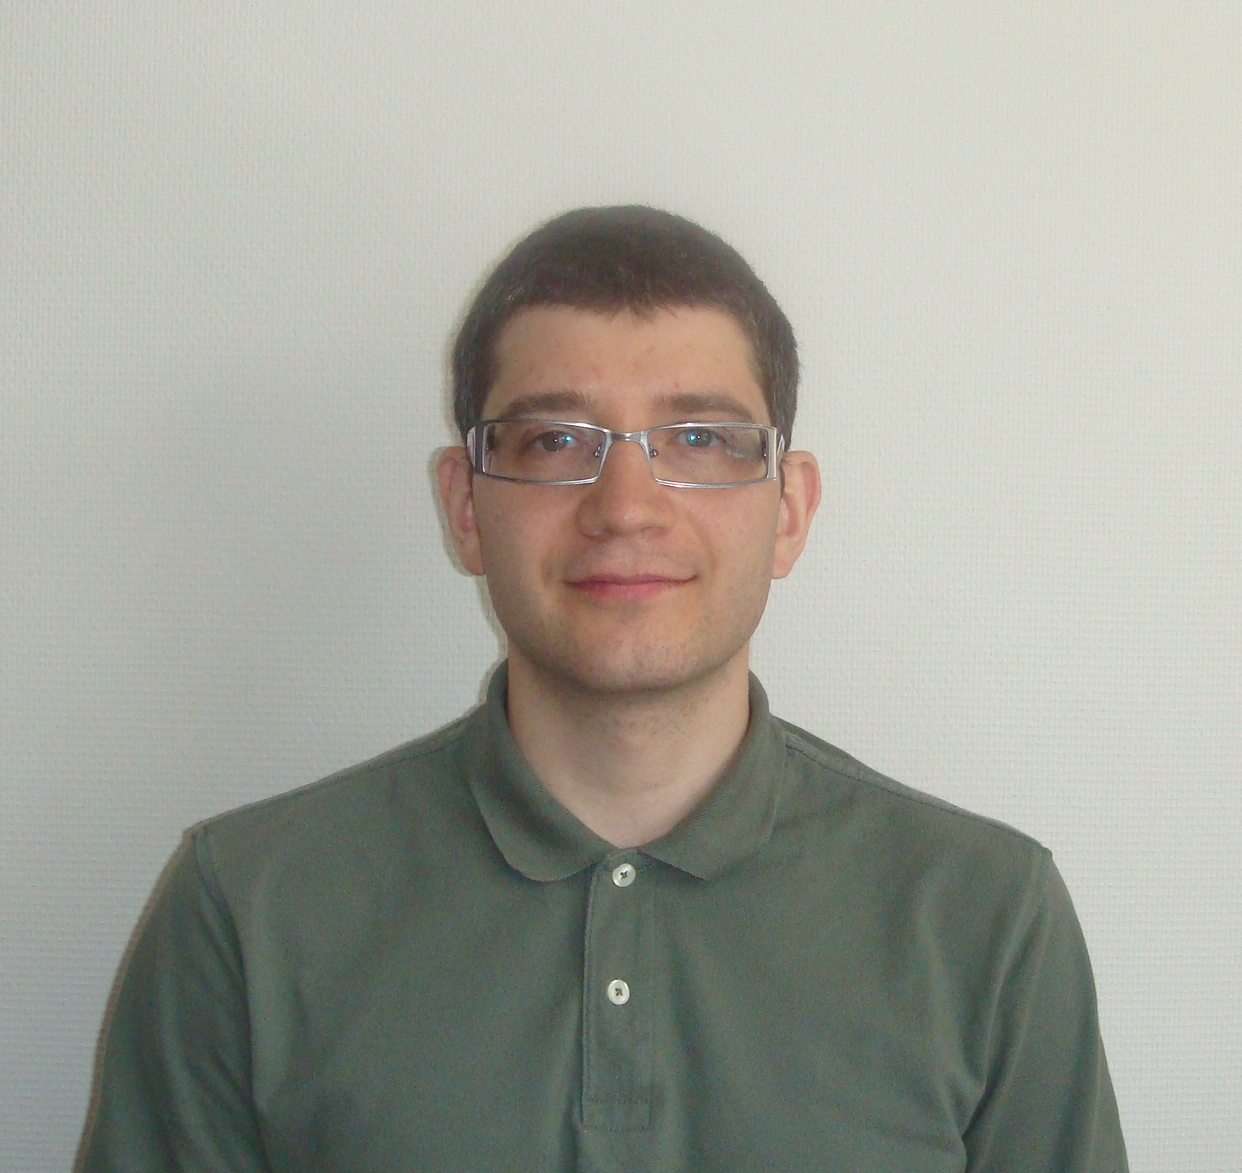
\includegraphics[width=4cm]{61_interv_2011_altoros.jpg}}
%\label{pic:fl1}
%\caption{Схема инфракрасного приемника}
%\end{figure}

За несколько дней до конференции организаторы пообщались с одним из докладчиков LVEE-2011, Алексеем Кондратенко. Алексей "--- активный контрибьютор в open source"=проекты, в частности Membase (Couchbase), а также ведущий разработчик Альторос Девелопмент. Во время беседы он поделился своими мыслями о выборе лицензий, тенденциях open source"=проектов, недавней поездке в Кремниевую долину и дал несколько советов начинающим Linux"=разработчикам.

{\noindent \bf LVEE: Алексей, расскажи немного о себе.}

{\noindent \bf Алексей:} Программирую. Много.

{\noindent \bf L:  В каких свободных проектах ты принимал участие?}

{\noindent \bf A:} Мне довелось портировать один полупроприетарный драйвер программного модема в Linux 2.6. Я поучаствовал немного в разработке Ruby on Rails, а также написал замечательный навигатор по проекту и документации (gpicker). Но, разумеется, самое значительное, "--- это  мое участие в проекте Membase. И особенно приятно, что это работа за деньги, но над free software.
 
{\noindent \bf L:  Какой из этих проектов тебе наиболее интересен с профессиональной точки зрения?}

{\noindent \bf A:} В каждом проекте или проектике есть свои изюминки. Я считаю, что не бывает неинтересных задач. Бывают только неинтереснее решения. Я считаю, что очень важно научиться получать удовольствие от качественно сделанной работы. Тогда любая, даже самая тривиальная задача, будет приносить удовольствие. В компании, где я работаю, созданы именно такие условия для самореализации.

{\noindent \bf L:  Расскажи нам о своем мнении по поводу основных лицензий для распространения ПО. Сдерживают ли по"=твоему лицензионные ограничения развитие open source"=продуктов?}

{\noindent \bf A:} Два больших и очень различных класса "--- это copyleft и non-copyleft лицензии.

Первый класс представляют лицензии вроде GPL, LGPL и AGPL. Эти лицензии обеспечивают публичность модификаций. GPL, например, требует, чтобы параллельно с предоставлением готовой программы (оригинальной или модифицированной) предоставлялся доступ к исходным кодам. Это не позволяет всяким жадным корпорациям развивать свои закрытые форки. К сожалению, я был свидетелем того, как люди,  на мой взгляд неоправданно, опасаются этого класса лицензий. Я слышал, будто бы GPL"=код помешал покупке нескольких стартапов. Всем известно, что Android практически целиком избегает GPL (кроме неизбежного GPL для kernel).

Второй класс не накладывает copyleft"=ограничений. Он позволяет компаниям «наживаться» на своих закрытых версиях open source"=проектов. Хотя обычно скрывать код и форкать его не очень выгодно. Так что сторонники этого класса лицензий как правило упирают на большую либеральность. Сама возможность делать с кодом все что угодно "= большой плюс для них.

Конечно, copyleft versus non"=copyleft являются только одной гранью различия лицензий. Есть еще много всяких тонкостей, например, борьба против DRM и патентная волокита.

Выбор лицензии (или смена ее) может быть поводом для создания альтернативного проекта с более мягкой лицензией. Например, компания Apple полным ходом идет к отказу от GPL"=ного GCC в пользу основанного на LLVM набора компиляторов Clang. Сейчас они поставляют очень древние версии gcc, gdb и других частей gnu toolchain. Одной из причин является переход данных проектов на GPL версии 3. Также есть основания полагать, что Apple готовит альтернативу Samba, которая тоже перешла на GPL3.

 
{\noindent \bf L:  Поделись своими мыслями, за счёт чего идёт развитие open source"=проектов? В смысле финансовой стороны.}

{\noindent \bf A:} Есть разные модели зарабатывания денег на free software. В последнее время большее распространение получает модель, при которой клиенты покупают не сам софт, а подписку на поддержку. RedHat довольно успешно зарабатывает миллиарды в год на этой модели.

Но голый энтузиазм никогда не пропадет полностью. На github, например, можно найти кучу очень впечатляющих проектов, которые люди делают в свое личное время.


{\noindent \bf L:  Как ты считаешь, при сравнении open source"=проектов с коммерческими, в каком случае качество проигрывает и почему?}

{\noindent \bf A:} Я считаю, что это независимые вещи. Можно одинаково хорошо или плохо делать и свободный и проприетарный софт. Свободный софт дает мне ряд возможностей: видеть, что внутри, исправлять это, и наконец, использовать его куски в других проектах. 

Но качество всегда определяется личностными характеристиками и упорством инженеров, которые над кодом работают.

{\noindent \bf L:  Всегда ли open source"=проекты бесплатны?}

{\noindent \bf A:} И да, и нет. Всегда можно просто взять и применить любой свободный софт. Но внедрение любых технологий в организациях требует некоторых затрат на обучение/поддержку и так далее. И этого невозможно избежать.


{\noindent \bf L:  Какое, на твой взгляд, будущее ждет open source"=проекты?}

{\noindent \bf A:} Теперь уже очевидно, что open source "--- это просто часть мейнстрима. Будущее таких важных инициатив как GNU Linux (особенно на десктопах) по"=прежнему не очевидно. Но сам факт повседневного применения свободного софта уже является неотъемлемой частью нашего программистского дела. Да, в принципе, и повседневного быта обычных людей.

Также очень ценной является доступность кода фреймворка или библиотеки, которую используешь. Похоже, что не только я один привык иметь возможность «копать» сколь угодно глубоко, разбираясь с какой-либо проблемой. Это связано с тем, что очень часто баги встречаются «на стыке» технологий.

Сейчас все меньше остается проприетарных и закрытых технологий (а интересных так и вообще нет). Я думаю, что люди просто все больше привыкают полагаться на наличие кода. И совсем скоро это будет просто must have.

{\noindent \bf L:  Чем ты пользуешься в работе?}

{\noindent \bf A:} Я большой сторонник GNU/Linux ифилософии free software в частности. Для работы использую Emacs и кучу великолепных маленьких утилит и утилиток, которыми так славен free software world.

{\noindent \bf L:  Книга которую должен прочесть каждый программист?}

{\noindent \bf A:} Сложно сказать. Есть множество очень классных книжек, которые можно рекомендовать по разным причинам. Думаю «классический» выбор в пользу TAOCP и SICP никого не удивит.

{\noindent \bf L:  А без какой художественной книги ты бы не стал программистом?}

{\noindent \bf A:} Я стал программистом не из"=за художественной литературы. Когда я был в третьем классе, отец собрал Baltic. Это советский клон культового ZX Spectrum. Играть на нем, разумеется, было очень интересно. Потом у меня начали получаться простые программки, из которых постепенно и вырос интерес к программированию.

{\noindent \bf L:  Какой профессиональный совет ты можешь дать начинающим программистам?}

{\noindent \bf A:} Я вижу, как люди сталкиваясь с проблемами, скажем, в Rails или в каком"=либо плагине, не проявляют должной активности для доведения их исправления до upstream. Иногда разработчики  отправляют патчи, которые потом просто пропадают. Очень важно понять, что правильный и завершенный фикс надо еще правильно оформить и подать людям, которые отвечают за проект. И это также очень важная и непростая работа. Главное "--- это не бояться и помнить, что в любом проекте есть правила подачи патчей. Если все делать правильно и не сдаваться, то эффект будет не только для самолюбия, но и для всего человечества, как бы пафосно это ни звучало.

{\noindent \bf L:  Алексей, ты только что вернулся из Кремниевой долины в Калифорнии, самой Мекки программистов. Как впечатления? Расскажи, где тебе работалось лучше.}

{\noindent \bf A:} Непосредственно работа там получается лучше. Наверное, это обусловлено тем, что полностью отсутствуют отвлекающие факторы. Мне вот, например, удалось прилично похудеть благодаря смене обстановки и отсутствию наивкуснейшей домашней пищи.

А в целом же, большой разницы с работой, например, в офисе Altoros не почувствовал. Но здесь мне однозначно нравиться больше. Трава точно зеленее. И девушки на порядок красивее :)



\end{document}


